\documentclass[10pt]{report}

\usepackage{geometry}
\geometry{
	a4paper,
	margin=1in,
	footskip=0.25in
}

\usepackage{enumerate} % for enumerate counter
\usepackage{subcaption} % for subfigures
\usepackage{amsthm} % for QED
\usepackage{mathtools} % for delimiter

\usepackage{listings} % for code
\lstset{ 
	language=R,
	basicstyle=\footnotesize\ttfamily,
	numbers=none,
	stepnumber=1,
	numbersep=8pt,
	showspaces=false,
	showstringspaces=false,
	showtabs=false,
	frame=single,
	tabsize=2,
	captionpos=t,
	breaklines=true,
	breakatwhitespace=false
} 

\usepackage{float} % for figure [H]
\usepackage{booktabs} % for tabular
\usepackage{caption} % for \caption*
\usepackage[export]{adjustbox} % for valign=t
\usepackage{array} % for column type m
\usepackage{verbatim}
\usepackage{graphicx}
%\graphicspath{ {imgs/} }

\usepackage{fancyhdr}
\pagestyle{fancy}
\fancyhead[L]{\hwAuther}
\fancyhead[C]{\courseNo}
\fancyhead[R]{\hwNo}

\usepackage{amssymb}
\usepackage{amsmath}

%Cover
\newcommand{\courseTitle}{Introduction to Mathematical Modeling}
\newcommand{\courseNo}{Math 380}
\newcommand{\hwAuther}{Zhihao Ai}

\newcommand{\hwNo}{HW \#3}
\newcommand{\hwDate}{Due on 02/13}

\title{
	\courseTitle\\
	\hwNo\\
	\hwDate
}
\author{\hwAuther}
\date{}
%

%Custom
%\everymath{\displaystyle}
\setlength\parindent{0pt}

%Custom commands
\newcommand{\ds}{\displaystyle}
\newcommand{\ts}{\textstyle}

\newcolumntype{N}{>$ c <$} 
\newcolumntype{M}[1]{>{\centering\arraybackslash $}m{#1}<{$}}

\newcommand{\abs}[1] {\left| #1 \right|}

\DeclarePairedDelimiter\autoparen{(}{)}
\newcommand{\pa}[1]{\autoparen*{#1}}

\newcommand{\var} {\text{var}}

\newcommand{\m}[1] {\mathbf{#1}}

\begin{document}

\maketitle

\section*{Section 3.1}
\begin{enumerate}
	\item [5.]
	The following data represent the growth of a population of fruit flies over a 6-week period. Test the following models by plotting an appropriate set of data. Estimate the parameters of the following models.
	\begin{table}[H]
		\centering
		\begin{tabular}{*{7}{c}} 
			\toprule
			$t$ (days) & 7 & 14 & 21 & 28 & 35 & 42 \\ \midrule
			$P$ (number of observed flies) & 8 & 41 & 133 & 250 & 280 & 297 \\
			\bottomrule
		\end{tabular}
	\end{table}
	\begin{enumerate}[a.]
		\item 
		$P = c_1 t$
		
		Plotting $P$ against $t$, we have
		\begin{figure}[H]
			\centering
			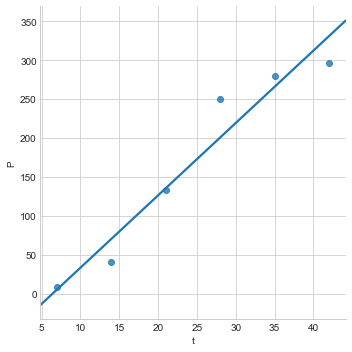
\includegraphics[width=0.4\linewidth]{s3_1/5a.png}
		\end{figure}
		$c_1$ is estimated to be $\frac{133-8}{21-7} = 8.93$.
	
		\item 
		$P = a e^{bt}$
		
		Plotting $\ln{P}$ against $t$, we have
		\begin{figure}[H]
			\centering
			\begin{subfigure}[b]{.4\linewidth}
				\caption{$\ln{P}$ vs $t$}
				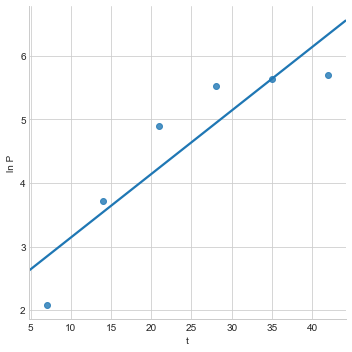
\includegraphics[width=\linewidth]{s3_1/5b.png}
			\end{subfigure}%%
			\begin{subfigure}[b]{.4\linewidth}
				\caption{Fitted model}
				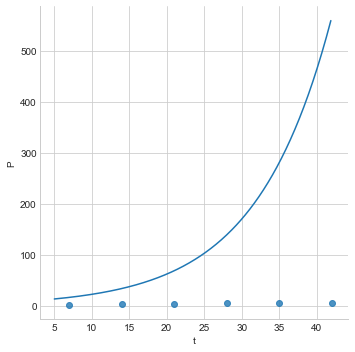
\includegraphics[width=\linewidth]{s3_1/5bo.png}
			\end{subfigure}
		\end{figure}
		Since $\ln{P} = \ln{a} + bt$, $\ln{a}$ is estimated to be 2.7 so $a$ is about 14.88 and $b$ is estimated to be 0.1. This model is not a good fit when plotting $ a e^{bt}$ against $t$.
	\end{enumerate}

	\item [7.]
	In 1601 the German astronomer Johannes Kepler became director of the Prague Observatory. Kepler had been helping Tycho Brahe in collecting 13 years of ovservations on the relative motion of the planet Mars. By 1609 Kepler had formulated his first two laws. Kepler spent many years verifying these laws and formulating a third law, which relates the planets' orbital periods and mean distances from the sun.
	\begin{enumerate}[a.]
		\item 
		Plot the period time $T$ versus the mean distance $r$ using the observational data.
		\begin{figure}[H]
			\centering
			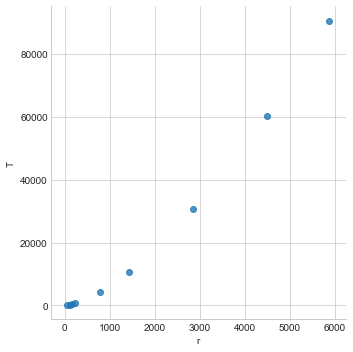
\includegraphics[width=0.4\linewidth]{s3_1/7a.png}
		\end{figure}
		
		\item 
		Assuming a relationship of the form
		\[
		T = C r^a
		\]
		determine the parameters $C$ and $a$ by plotting $\ln{T}$ versus $\ln{r}$. Does the model seem reasonable? Try to formulate Kepler's third law.
		\begin{figure}[H]
			\centering
			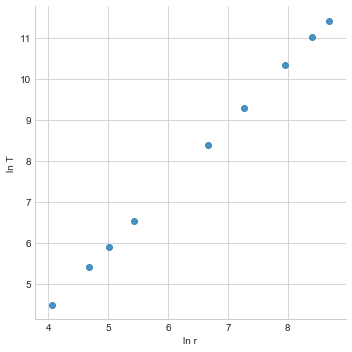
\includegraphics[width=0.4\linewidth]{s3_1/7b.png}
		\end{figure}
		Since $\ln{T} = \ln{C} + a \ln{r}$, $\ln{C}$ is estimated to be $-1.62$ so $C$ is about 0.2 and $a$ is estimated to be 1.5. Kepler's third law would be the planets' orbital periods are proportional to the mean distances from the sun to the power 1.5, or mathematically, $T = 0.2 r^{1.5}$.
	\end{enumerate}
\end{enumerate}

\section*{Section 3.2}
\begin{enumerate}
	\item [2b.]
	Formulate the mathematical model that minimizes the largest deviation between the data and the line $y=ax+b$. Solve for the estimates of $a$ and $b$.
	\begin{table}[H]
		\centering
		\begin{tabular}{*{9}{c}} 
			\toprule
			$x$ & 29.1 & 48.2 & 72.7 & 92.9 & 118 & 140 & 165 & 199\\ \midrule
			$y$ & 0.0493 & 0.0821 & 0.123 & 0.154 & 0.197 & 0.234 & 0.274 & 0.328 \\
			\bottomrule
		\end{tabular}
	\end{table}
	If $r$ represents the largest absolute value of the residuals, the problem is to
	\[
	\text{Minimize } r
	\]
	subject to
	\begin{align*}
		r - (29.1a + b - 0.0493) &\ge 0\\
		r + (29.1a + b - 0.0493) &\ge 0\\
		r - (48.2 a + b - 0.0821) &\ge 0\\
		r + (48.2 a + b - 0.0821) &\ge 0\\
		r - (72.7 a + b - 0.123) &\ge 0\\
		r + (72.7 a + b - 0.123) &\ge 0\\
		r - (92.9 a + b - 0.154) &\ge 0\\
		r + (92.9 a + b - 0.154) &\ge 0\\
		r - (118 a + b - 0.197) &\ge 0\\
		r + (118 a + b - 0.197) &\ge 0\\
		r - (140 a + b - 0.234) &\ge 0\\
		r + (140 a + b - 0.234) &\ge 0\\
		r - (165 a + b - 0.274) &\ge 0\\
		r + (165 a + b - 0.274) &\ge 0 \\
		r - (199 a + b - 0.328) &\ge 0 \\
		r + (199 a + b - 0.328) &\ge 0
	\end{align*}
	Using Mathematica, $r$ is minimized when $a=0.00164038$ and $b=0.00295615$.
	
	\item [3.]
	For the following data, formulate the mathematical model that minimizes the largest deviation between the data and the model $y = c_1 x^2 + c_2 x + c_3$. Solve for the estimates of $c_1$, $c_2$ and $c_3$.
	\begin{table}[H]
		\centering
		\begin{tabular}{*{6}{c}} 
			\toprule
			$x$ & 0.1 & 0.2 & 0.3 & 0.4 & 0.5 \\ \midrule
			$y$ & 0.06 & 0.12 & 0.36 & 0.65 & 0.95 \\
			\bottomrule
		\end{tabular}
	\end{table}
	If $r$ represents the largest absolute value of the residuals, the problem is to
	\[
	\text{Minimize } r
	\]
	subject to
	\begin{align*}
	r - (0.1^2 c_1 + 0.1 c_2 + c_3 - 0.06) &\ge 0\\
	r + (0.1^2 c_1 + 0.1 c_2 + c_3 - 0.06) &\ge 0\\
	r - (0.2^2 c_1 + 0.2 c_2 + c_3 - 0.12) &\ge 0\\
	r + (0.2^2 c_1 + 0.2 c_2 + c_3 - 0.12) &\ge 0\\
	r - (0.3^2 c_1 + 0.3 c_2 + c_3 - 0.36) &\ge 0\\
	r + (0.3^2 c_1 + 0.3 c_2 + c_3 - 0.36) &\ge 0\\
	r - (0.4^2 c_1 + 0.4 c_2 + c_3 - 0.65) &\ge 0\\
	r + (0.4^2 c_1 + 0.4 c_2 + c_3 - 0.65) &\ge 0\\
	r - (0.5^2 c_1 + 0.5 c_2 + c_3 - 0.95) &\ge 0\\
	r + (0.5^2 c_1 + 0.5 c_2 + c_3 - 0.95) &\ge 0
	\end{align*}
	Using Mathematica, $r$ is minimized when $c_1=4$, $c_2=-0.0333$ and $c_3=-0.005$.
\end{enumerate}

\end{document}

